\chapter{Ciclos de vida y reproducción de las plantas terrestres}\label{ch:b2:plant-life-cycles}

El cojín verde de \omterm{def:b2:plant-life-cycles:moss}{musgo} sobre un muro es una planta; los tallitos pardos
que brotan de él en primavera, cada uno con una cápsula de esporas, son
otra --- un individuo distinto, con el doble de cromosomas, que crece a
partir del primero y vive sobre él. La fronda de un \omterm{def:b2:plant-life-cycles:fern}{helecho} lleva esporas
en su cara inferior, pero las esporas no dan \omterm{def:b2:plant-life-cycles:fern}{helechos}: dan una lámina
verde con forma de corazón de unos pocos milímetros de ancho, que es
donde se forman los anterozoides y las oosferas, y es de esa lámina de
donde brota un nuevo \omterm{def:b2:plant-life-cycles:fern}{helecho}. Toda planta terrestre alterna así entre dos
cuerpos, uno \omterm{def:b2:meiosis-heredity:meiosis}{haploide} y otro \omterm{def:b2:meiosis-heredity:meiosis}{diploide}. Este capítulo sigue esa
alternancia desde las algas hasta la semilla, y muestra cómo una serie de
cambios --- la reducción del cuerpo \omterm{def:b2:meiosis-heredity:meiosis}{haploide}, la invención del \omterm{def:b2:plant-life-cycles:heterospory}{polen}, el
encierro del \omterm{def:b2:plant-life-cycles:heterospory}{óvulo}, la semilla --- liberó la reproducción del agua y
permitió a las plantas cubrir los continentes.

\section{Tres tipos de ciclo de vida}

\begin{definition}[Haplonte, diplonte, haplodiplonte]\label{def:b2:plant-life-cycles:cycles}
\index{ciclo de vida}\index{alternancia de generaciones}\index{gametofito}\index{esporofito}
Todo ciclo de vida sexual contiene una \emph{fecundación}, que duplica el
número de cromosomas, y una \emph{\omterm{def:b2:meiosis-heredity:meiosis}{meiosis}}, que lo reduce a la mitad; los
ciclos difieren en lo que ocurre entre ambas. En un ciclo
\emph{haplonte} el cigoto es la única célula \omterm{def:b2:meiosis-heredity:meiosis}{diploide} y sufre la \omterm{def:b2:meiosis-heredity:meiosis}{meiosis}
de inmediato; el organismo es \omterm{def:b2:meiosis-heredity:meiosis}{haploide} y sus gametos se forman por
mitosis (\emph{Chlamydomonas}, muchas algas y hongos). En un ciclo
\emph{diplonte} la \omterm{def:b2:meiosis-heredity:meiosis}{meiosis} produce directamente los gametos, que son las
únicas células \omterm{def:b2:meiosis-heredity:meiosis}{haploides}, y el organismo es \omterm{def:b2:meiosis-heredity:meiosis}{diploide} (los animales, el
alga parda \emph{Fucus}). En un ciclo \emph{haplodiplonte} la \omterm{def:b2:meiosis-heredity:meiosis}{meiosis}
produce \emph{esporas}, que por mitosis dan un organismo \omterm{def:b2:meiosis-heredity:meiosis}{haploide}, el
\emph{gametofito}, que forma los gametos por mitosis; el cigoto da por
mitosis un organismo \omterm{def:b2:meiosis-heredity:meiosis}{diploide}, el \emph{esporofito}, que forma las
esporas por \omterm{def:b2:meiosis-heredity:meiosis}{meiosis}. Se alternan dos cuerpos \omterm{def:b2:unicellular-diversity:unicellular}{pluricelulares} --- la
\emph{alternancia de generaciones} ---, y este es el ciclo de todas las
plantas terrestres y de muchas algas.
\end{definition}

\begin{omfigure}
\begin{tikzpicture}[every node/.style={font=\scriptsize}, >=stealth]
  \foreach \dx/\title/\hap/\dip in {0/{haplonte (\emph{Chlamydomonas})}/{organismo haploide ($n$)}/{cigoto ($2n$)}, 5.2/{diplonte (animales)}/{gametos ($n$)}/{organismo diploide ($2n$)}, 10.4/{haplodiplonte (plantas)}/{gametofito ($n$)}/{esporofito ($2n$)}} {
    \begin{scope}[xshift=\dx cm]
      \node[anchor=south, font=\scriptsize\bfseries] at (2,2.5) {\title};
      \draw[thick, omDef, ->] (0.6,0.4) arc (200:340:1.5 and 1.0);
      \draw[thick, omThm, ->] (3.4,1.4) arc (20:160:1.5 and 1.0);
      \node[omDef, anchor=north] at (2,-0.3) {\hap};
      \node[omThm, anchor=south] at (2,2.05) {\dip};
      \node[anchor=south west] at (3.4,1.05) {fecundación};
      \node[anchor=north east] at (0.55,0.75) {meiosis};
    \end{scope}
  }
  % emphasise the dominant phase by thickness of the arcs: draw thicker arcs
  \draw[line width=2.4pt, omDef, ->] (0.6,0.4) arc (200:340:1.5 and 1.0);
  \draw[line width=2.4pt, omThm, ->] (5.2+3.4,1.4) arc (20:160:1.5 and 1.0);
  \draw[line width=2.4pt, omDef, ->] (10.4+0.6,0.4) arc (200:340:1.5 and 1.0);
  \draw[line width=2.4pt, omThm, ->] (10.4+3.4,1.4) arc (20:160:1.5 and 1.0);
\end{tikzpicture}

{\small Tres \omterm{def:b2:plant-life-cycles:cycles}{ciclos de vida}. En azul, la fase \omterm{def:b2:meiosis-heredity:meiosis}{haploide}; en rojo, la fase
\omterm{def:b2:meiosis-heredity:meiosis}{diploide}; los arcos gruesos son los cuerpos \omterm{def:b2:unicellular-diversity:unicellular}{pluricelulares}. Todo ciclo
pasa una vez por la \omterm{def:b2:meiosis-heredity:meiosis}{meiosis} y una vez por la fecundación; difieren en qué
fase --- o ambas --- crece hasta formar un organismo.}
\end{omfigure}

\begin{proposition}[Qué significa la alternancia de generaciones]\label{prop:b2:plant-life-cycles:alternation}
En una planta terrestre las dos generaciones son dos organismos, no dos
etapas de uno solo: el \omterm{def:b2:plant-life-cycles:cycles}{gametofito} y el \omterm{def:b2:plant-life-cycles:cycles}{esporofito} tienen genomas
distintos (\omterm{def:b2:meiosis-heredity:meiosis}{haploide} y \omterm{def:b2:meiosis-heredity:meiosis}{diploide}), cuerpos distintos, a menudo tamaños que
difieren en órdenes de magnitud, y cada uno se desarrolla por mitosis a
partir de una sola célula --- una espora o un cigoto. El \omterm{def:b2:plant-life-cycles:cycles}{gametofito} forma
los gametos en órganos \omterm{def:b2:unicellular-diversity:unicellular}{pluricelulares}, los \emph{\omterm{def:b2:plant-life-cycles:moss}{anteridios}}
(anterozoides) y los \emph{\omterm{def:b2:plant-life-cycles:moss}{arquegonios}} (una oosfera cada uno, en un
matraz por cuyo cuello desciende nadando el anterozoide); el
\omterm{def:b2:plant-life-cycles:cycles}{esporofito} forma las esporas en \emph{\omterm{def:b2:plant-life-cycles:fern}{esporangios}}. A lo largo de las
plantas terrestres el equilibrio se desplaza: en los \omterm{def:b2:plant-life-cycles:moss}{musgos} el \omterm{def:b2:plant-life-cycles:cycles}{gametofito}
es la planta y el \omterm{def:b2:plant-life-cycles:cycles}{esporofito} un tallito dependiente; en los \omterm{def:b2:plant-life-cycles:fern}{helechos} el
\omterm{def:b2:plant-life-cycles:cycles}{esporofito} es la planta y el \omterm{def:b2:plant-life-cycles:cycles}{gametofito} una lámina de vida libre; en las
plantas con semilla el \omterm{def:b2:plant-life-cycles:cycles}{gametofito} queda reducido a unas pocas células
ocultas en los tejidos del \omterm{def:b2:plant-life-cycles:cycles}{esporofito} --- el grano de \omterm{def:b2:plant-life-cycles:heterospory}{polen} y el
contenido del \omterm{def:b2:plant-life-cycles:heterospory}{óvulo}.
\end{proposition}
\begin{proof}[Evidencia]
Hofmeister (1851) hizo germinar esporas de \omterm{def:b2:plant-life-cycles:moss}{musgos}, \omterm{def:b2:plant-life-cycles:fern}{helechos}, equisetos y
licopodios, siguió el desarrollo de los pequeños cuerpos verdes que
producían, encontró en ellos los \omterm{def:b2:plant-life-cycles:moss}{anteridios} y los \omterm{def:b2:plant-life-cycles:moss}{arquegonios}, y vio
crecer el embrión desde la oosfera fecundada, dentro del \omterm{def:b2:plant-life-cycles:moss}{arquegonio}, hasta
la planta portadora de esporas. Mostró después que el \omterm{def:b2:plant-life-cycles:heterospory}{óvulo} de una
conífera contiene las mismas estructuras, reducidas --- \omterm{def:b2:plant-life-cycles:moss}{arquegonios}
dentro de un tejido que es un \omterm{def:b2:plant-life-cycles:cycles}{gametofito} retenido ---, y por tanto que
\omterm{def:b2:plant-life-cycles:moss}{musgos}, \omterm{def:b2:plant-life-cycles:fern}{helechos} y plantas con semilla forman una sola serie con un solo
ciclo. Los recuentos de cromosomas que explicaron las dos generaciones
(Strasburger, 1894) llegaron cuarenta años después.
\end{proof}

\section{Los musgos: el gametofito es la planta}

\begin{definition}[El ciclo de vida del musgo]\label{def:b2:plant-life-cycles:moss}
\index{musgo}\index{protonema}\index{arquegonio}\index{anteridio}
Una \emph{espora} de musgo germina y da un filamento verde ramificado, el
\emph{protonema}, del que brotan yemas que dan los tallos foliosos --- el
\emph{\omterm{def:b2:plant-life-cycles:cycles}{gametofito}}, de unos pocos centímetros de altura, sin verdaderas
raíces, xilema ni floema, fijado por rizoides y que absorbe agua por toda
su superficie. En el extremo de los tallos lleva \emph{anteridios}, que
liberan anterozoides biflagelados en una película de lluvia o de
rocío, y \emph{arquegonios}, cada uno con una oosfera en la base de un
cuello; los anterozoides nadan unos pocos centímetros como mucho,
guiados por atrayentes químicos, y fecundan la oosfera allí mismo. El
cigoto crece hasta formar el \emph{\omterm{def:b2:plant-life-cycles:cycles}{esporofito}}: un pie hundido en el
\omterm{def:b2:plant-life-cycles:cycles}{gametofito}, un pedicelo (\emph{seta}) y una \emph{cápsula} en la que la
\omterm{def:b2:meiosis-heredity:meiosis}{meiosis} produce decenas de miles de esporas, liberadas a través de un
anillo de dientes higroscópicos que se abren con el aire seco. El
\omterm{def:b2:plant-life-cycles:cycles}{esporofito} realiza un poco de fotosíntesis, pero el \omterm{def:b2:plant-life-cycles:cycles}{gametofito} lo
alimenta a través de su pie y nunca vive por sí solo.
\end{definition}

\begin{omfigure}
\begin{tikzpicture}[every node/.style={font=\scriptsize}, >=stealth]
  \node[draw, rounded corners, fill=omDef!12, align=center] (spore) at (0,3) {espora ($n$)};
  \node[draw, rounded corners, fill=omDef!12, align=center] (proto) at (3.2,3) {protonema};
  \node[draw, rounded corners, fill=omDef!12, align=center] (gam) at (6.6,3) {gametofito folioso ($n$)\\anteridios y arquegonios};
  \node[draw, rounded corners, fill=omDef!12, align=center] (gametes) at (11.2,3) {anterozoide y oosfera ($n$)};
  \node[draw, rounded corners, fill=omThm!12, align=center] (zyg) at (11.2,0.8) {cigoto ($2n$)};
  \node[draw, rounded corners, fill=omThm!12, align=center] (sporo) at (6.6,0.8) {esporofito ($2n$)\\pie, seta, cápsula};
  \node[draw, rounded corners, fill=omThm!12, align=center] (cap) at (2.4,0.8) {meiosis en la cápsula};
  \draw[->, thick] (spore) -- (proto) node[midway, above] {mitosis};
  \draw[->, thick] (proto) -- (gam);
  \draw[->, thick] (gam) -- (gametes) node[midway, above] {mitosis};
  \draw[->, thick] (gametes) -- (zyg) node[pos=0.3, right, align=left] {fecundación\\en una película de agua};
  \draw[->, thick] (zyg) -- (sporo) node[midway, above] {mitosis};
  \draw[->, thick] (sporo) -- (cap);
  \draw[->, thick] (cap) -| (spore) ;
  \node[omDef, anchor=west] at (-1.9,3.9) {haploide};
  \node[omThm, anchor=west] at (-1.9,-0.1) {diploide};
  \draw[gray, dashed] (-1.9,1.9) -- (13.2,1.9);
\end{tikzpicture}

{\small El ciclo del \omterm{def:b2:plant-life-cycles:moss}{musgo}. La planta foliosa es el \omterm{def:b2:plant-life-cycles:cycles}{gametofito} \omterm{def:b2:meiosis-heredity:meiosis}{haploide};
el \omterm{def:b2:plant-life-cycles:cycles}{esporofito} es un pedicelo con su cápsula que crece sobre él, alimentado
por él, y que forma esporas por \omterm{def:b2:meiosis-heredity:meiosis}{meiosis}.}
\end{omfigure}

\begin{omfigure}
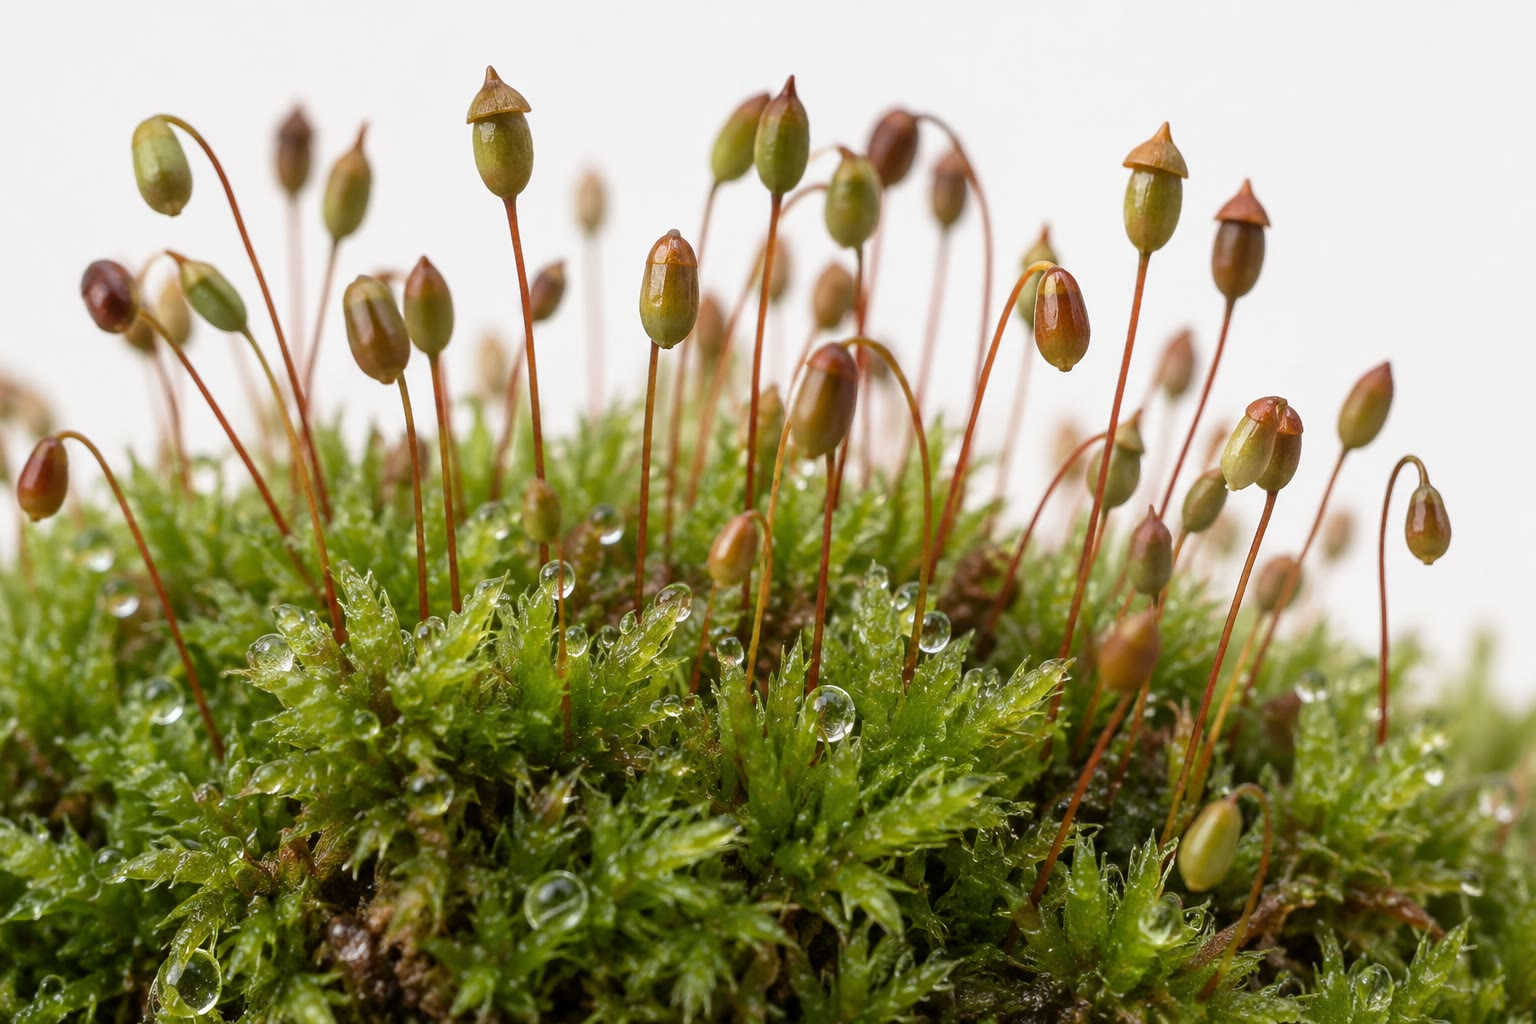
\includegraphics[width=0.6\linewidth]{images/book4/ai/b4-05-moss-sporophytes.jpg}

{\small Un cojín de \omterm{def:b2:plant-life-cycles:moss}{musgo} en primavera: los tallitos verdes son los
\omterm{def:b2:plant-life-cycles:cycles}{gametofitos}, y cada pedicelo rojizo con su cápsula es un \omterm{def:b2:plant-life-cycles:cycles}{esporofito}
nacido de una oosfera fecundada, todavía unido al tallo que produjo la
oosfera.}
\end{omfigure}

\begin{example}[El coste de los anterozoides nadadores]\label{ex:b2:plant-life-cycles:sperm}
Un anterozoide de \omterm{def:b2:plant-life-cycles:moss}{musgo} nada a unos \qty{100}{\micro m/s}; para
alcanzar un \omterm{def:b2:plant-life-cycles:moss}{arquegonio} situado a \qty{2}{cm} necesita \qty{200}{s} de
película de agua continua --- una salpicadura de lluvia, un rocío
abundante. La fecundación queda por tanto restringida al tiempo húmedo y
a distancias cortas, y la mayoría de los \omterm{def:b2:plant-life-cycles:moss}{musgos}, los \omterm{def:b2:plant-life-cycles:fern}{helechos} y sus
parientes viven en lugares húmedos o se reproducen en la estación de
lluvias; los \omterm{def:b2:plant-life-cycles:moss}{anteridios} de algunos \omterm{def:b2:plant-life-cycles:moss}{musgos} se sitúan en una copa de
salpicadura cuya forma lanza las gotas de lluvia, y los anterozoides
que llevan, a medio metro. Es de esta dependencia de la que escaparon las
plantas con semilla.
\end{example}

\section{Los helechos: el esporofito es la planta}

\begin{definition}[El ciclo de vida del helecho]\label{def:b2:plant-life-cycles:fern}
\index{helecho}\index{prótalo}\index{soro}\index{esporangio}
El helecho es el \emph{\omterm{def:b2:plant-life-cycles:cycles}{esporofito}}: un rizoma con raíces, xilema y floema,
y frondas. En la cara inferior de las frondas fértiles, grupos de
\emph{esporangios} (\emph{soros}, a menudo bajo una membrana protectora)
forman cada uno 64 esporas por \omterm{def:b2:meiosis-heredity:meiosis}{meiosis} y las lanzan con el chasquido de un
anillo de células de pared gruesa que se deseca. Una espora que cae en
suelo húmedo da un \emph{prótalo}: un \omterm{def:b2:plant-life-cycles:cycles}{gametofito} verde con forma de
corazón, de unos pocos milímetros de ancho y una sola célula de grosor,
con rizoides, que vive libre durante unas semanas. Lleva \omterm{def:b2:plant-life-cycles:moss}{anteridios} y
\omterm{def:b2:plant-life-cycles:moss}{arquegonios} en su cara inferior; los anterozoides nadan en la película
de agua del suelo hasta la oosfera; el cigoto da un \omterm{def:b2:plant-life-cycles:cycles}{esporofito} joven que
obtiene su primer alimento del prótalo y después echa raíces, y el
prótalo muere. Las dos generaciones son independientes, pero desiguales:
el \omterm{def:b2:plant-life-cycles:cycles}{esporofito} vive décadas y puede medir metros; el \omterm{def:b2:plant-life-cycles:cycles}{gametofito}, semanas y
milímetros.
\end{definition}

\begin{omfigure}
\begin{tikzpicture}[every node/.style={font=\scriptsize}, >=stealth]
  \node[draw, rounded corners, fill=omThm!12, align=center] (fern) at (0,3) {helecho, el esporofito ($2n$)\\raíces, rizoma, frondas};
  \node[draw, rounded corners, fill=omThm!12, align=center] (sor) at (5.4,3) {esporangios en soros\\(bajo las frondas)};
  \node[draw, rounded corners, fill=omDef!12, align=center] (spore) at (10.4,3) {esporas ($n$)\\64 por esporangio};
  \node[draw, rounded corners, fill=omDef!12, align=center] (pro) at (10.4,0.6) {prótalo ($n$)\\de vida libre, milimétrico\\anteridios, arquegonios};
  \node[draw, rounded corners, fill=omDef!12, align=center] (gam) at (5.4,0.6) {anterozoide y oosfera ($n$)};
  \node[draw, rounded corners, fill=omThm!12, align=center] (zyg) at (0,0.6) {cigoto ($2n$) y después\\esporofito joven\\sobre el prótalo};
  \draw[->, thick] (fern) -- (sor);
  \draw[->, thick] (sor) -- (spore) node[midway, above] {meiosis};
  \draw[->, thick] (spore) -- (pro) node[midway, right] {mitosis};
  \draw[->, thick] (pro) -- (gam) node[midway, above] {mitosis};
  \draw[->, thick] (gam) -- (zyg) node[midway, above, align=center] {fecundación\\(anterozoides nadadores)};
  \draw[->, thick] (zyg) -- (fern) node[midway, right] {mitosis};
  \draw[gray, dashed] (7.9,-0.5) -- (7.9,4.0);
  \node[omThm, anchor=south] at (2.7,3.9) {generación diploide};
  \node[omDef, anchor=south] at (10.4,3.9) {generación haploide};
\end{tikzpicture}

{\small El ciclo del \omterm{def:b2:plant-life-cycles:fern}{helecho}. La planta que llamamos \omterm{def:b2:plant-life-cycles:fern}{helecho} es el
\omterm{def:b2:plant-life-cycles:cycles}{esporofito} \omterm{def:b2:meiosis-heredity:meiosis}{diploide}; el \omterm{def:b2:plant-life-cycles:cycles}{gametofito} \omterm{def:b2:meiosis-heredity:meiosis}{haploide} es un \omterm{def:b2:plant-life-cycles:fern}{prótalo} de vida breve
sobre el que los anterozoides nadan hasta las oosferas.}
\end{omfigure}

\begin{omfigure}
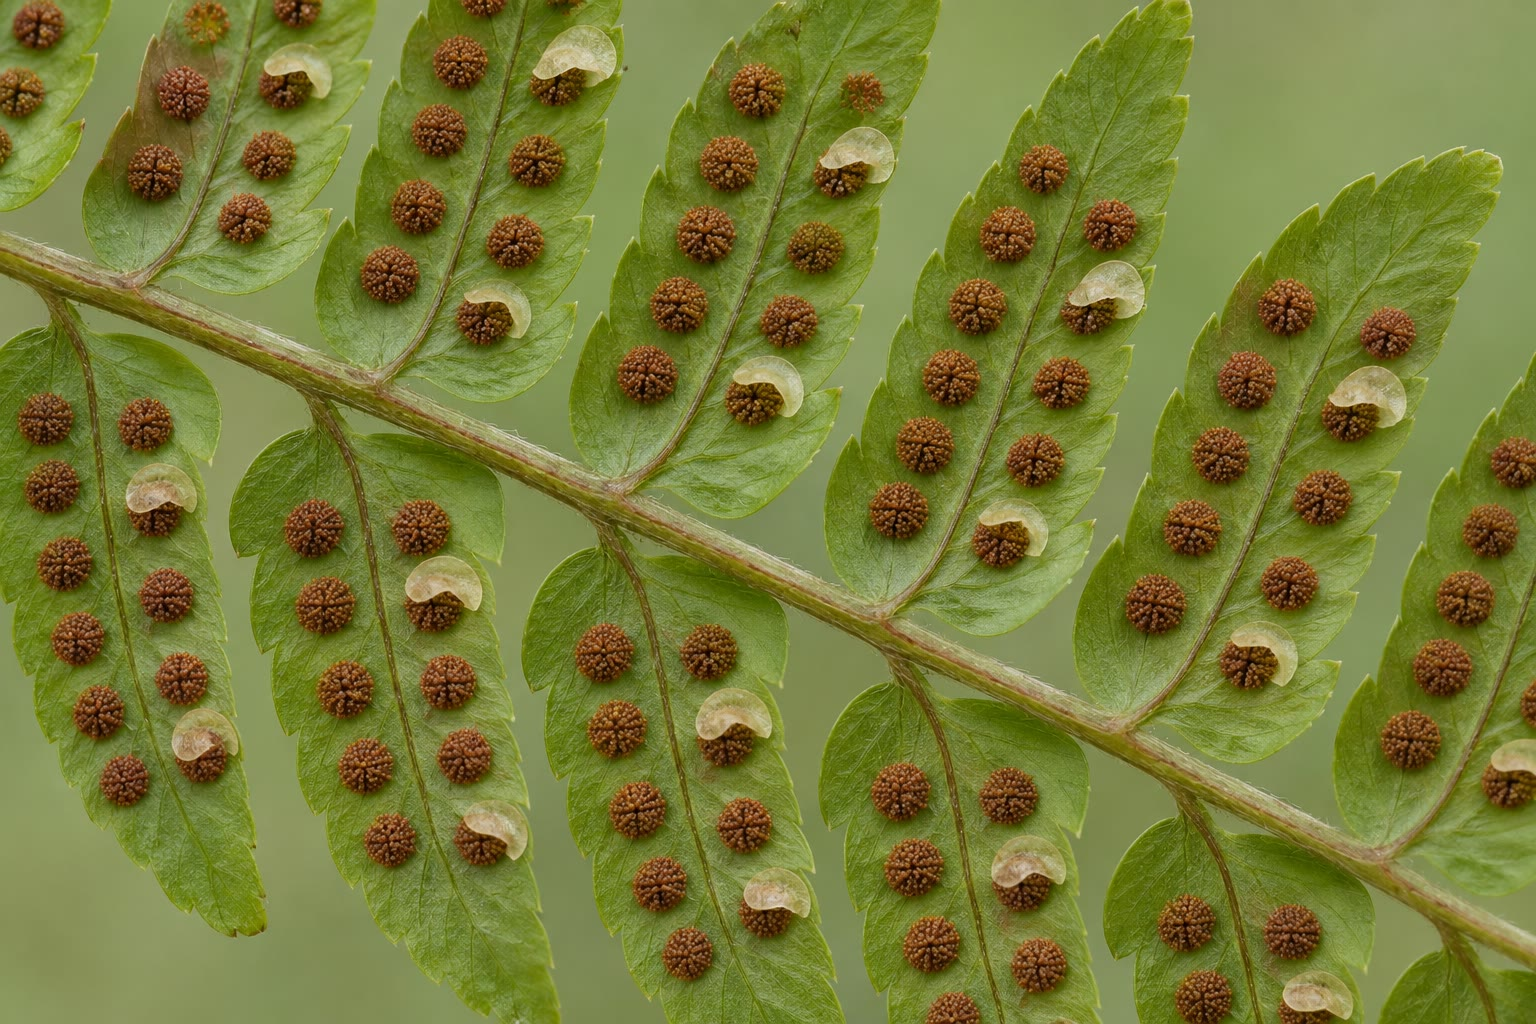
\includegraphics[width=0.6\linewidth]{images/book4/ai/b4-05-fern-sori.jpg}

{\small La cara inferior de una fronda fértil de \omterm{def:b2:plant-life-cycles:fern}{helecho}: cada punto pardo
es un \omterm{def:b2:plant-life-cycles:fern}{soro}, un grupo de \omterm{def:b2:plant-life-cycles:fern}{esporangios}, algunos todavía cubiertos por la
membrana que los protege hasta que maduran.}
\end{omfigure}

\begin{theorem}[Dispersión de una espora]\label{thm:b2:plant-life-cycles:dispersal}
\index{dispersión de las esporas}
Una espora de radio $r$ y densidad $\rho_s$ liberada a una altura $h$ en
un viento horizontal de velocidad $u$ cae a la velocidad límite de
Stokes
$v_s = 2r^2(\rho_s - \rho_{\text{aire}})g/9\eta_{\text{aire}}$
y aterriza, en aire estratificado en calma, a una distancia
\[
x = \frac{u\,h}{v_s}
\]
de la planta. Una espora de \omterm{def:b2:plant-life-cycles:fern}{helecho} de radio \qty{15}{\micro m} y
densidad \qty{1100}{kg/m^3} ($\eta_{\text{aire}} = \qty{1.8e-5}{Pa.s}$)
cae a \qty{3}{cm/s}; desde una fronda a \qty{0.5}{m}, con un viento de
\qty{2}{m/s}, recorre unos \qty{30}{m}, y en el aire turbulento de un día
ventoso, que eleva una fracción de las esporas muy por encima de la
altura de liberación, unas pocas recorren cientos de kilómetros --- por
eso las floras de \omterm{def:b2:plant-life-cycles:fern}{helechos} de las islas oceánicas son ricas y sus floras
de plantas con semilla, pobres.
\end{theorem}
\begin{proof}
El tiempo de caída es $h/v_s$ (la espora alcanza su velocidad límite en
microsegundos), durante el cual el viento la desplaza $u\,h/v_s$. La
velocidad límite se obtiene igualando el arrastre de Stokes $6\pi\eta r
v_s$ con el peso menos el empuje $\tfrac43\pi r^3(\rho_s -
\rho_{\text{aire}})g$, como en el \cref{ch:b2:unicellular-diversity}.
\end{proof}

\section{Las plantas con semilla: el gametofito oculto}

\begin{definition}[Heterosporia, polen, óvulo]\label{def:b2:plant-life-cycles:heterospory}
\index{heterosporia}\index{polen}\index{óvulo}\index{microspora}\index{megaspora}
Los \omterm{def:b2:plant-life-cycles:moss}{musgos} y la mayoría de los \omterm{def:b2:plant-life-cycles:fern}{helechos} son \emph{homospóricos}: un solo
tipo de espora, un solo tipo de \omterm{def:b2:plant-life-cycles:cycles}{gametofito} que lleva ambos sexos. Las
plantas con semilla (y algunos \omterm{def:b2:plant-life-cycles:fern}{helechos} y licopodios) son
\emph{heterospóricas}: las \emph{microsporas}, pequeñas y numerosas, dan
\omterm{def:b2:plant-life-cycles:cycles}{gametofitos} masculinos; las \emph{megasporas}, grandes y escasas,
\omterm{def:b2:plant-life-cycles:cycles}{gametofitos} femeninos. En las plantas con semilla ambos quedan reducidos
casi a nada y ninguno abandona por sí solo los tejidos del \omterm{def:b2:plant-life-cycles:cycles}{esporofito}. El
\omterm{def:b2:plant-life-cycles:cycles}{gametofito} masculino es el \emph{grano de polen}: una microspora que se ha
dividido dos o tres veces dentro de su pared, transportada por el viento
o por animales hasta el órgano femenino, donde forma un \emph{tubo
polínico} y entrega sus gametos masculinos --- sin necesidad de agua. El
\omterm{def:b2:plant-life-cycles:cycles}{gametofito} femenino se desarrolla dentro del megasporangio, que permanece
sobre la planta madre envuelto en uno o dos \emph{tegumentos} con un
poro, el \emph{micrópilo}: el conjunto es el \emph{óvulo}. Tras la
fecundación el óvulo se convierte en la \emph{semilla}: un \omterm{def:b2:plant-life-cycles:cycles}{esporofito}
embrionario, una reserva de alimento y una cubierta formada por los
tegumentos, en latencia hasta que las condiciones son favorables.
\end{definition}

\begin{omfigure}
\begin{tikzpicture}[every node/.style={font=\scriptsize}]
  % ovule in section
  \draw[thick, fill=omExo!25] (0,0) ellipse (1.6 and 2.2);
  \draw[thick, fill=omExo!10] (0,0) ellipse (1.25 and 1.85);
  \draw[thick, fill=white] (0,-0.15) ellipse (0.8 and 1.3);
  \draw[thick, fill=omDef!25] (0,0.6) ellipse (0.45 and 0.55);
  \fill[omDef!80!black] (0,0.75) circle (0.12);
  % micropyle: gap at top
  \fill[white] (-0.35,1.7) rectangle (0.35,2.35);
  \draw[thick] (-0.35,1.7) -- (-0.35,2.2); \draw[thick] (0.35,1.7) -- (0.35,2.2);
  \draw[thick] (-0.35,2.2) arc (180:90:0.1) ; \draw[thick] (0.35,2.2) arc (0:90:0.1);
  % pollen grain and tube
  \draw[thick, fill=omProp!40] (0.9,3.0) circle (0.22);
  \draw[thick, omProp] (0.75,2.85) .. controls (0.2,2.6) and (0.05,2.0) .. (0.05,1.25);
  % stalk
  \draw[thick] (0,-2.2) -- (0,-2.8);
  % labels
  \draw (1.45,-0.9) -- (2.6,-0.9) node[right] {tegumento(s)};
  \draw (1.0,-0.6) -- (2.6,-1.5) node[right] {megasporangio (nucela)};
  \draw (0.55,-1.0) -- (2.6,-2.1) node[right, align=left] {gametofito femenino\\(de una megaspora)};
  \draw (0.35,0.45) -- (2.6,0.3) node[right] {arquegonio};
  \draw (0.1,0.78) -- (2.6,1.0) node[right] {oosfera};
  \draw (0.35,2.0) -- (2.6,2.0) node[right] {micrópilo};
  \draw (1.1,3.0) -- (2.6,3.0) node[right] {grano de polen y tubo polínico};
  \node[right] at (0.1,-2.6) {pedúnculo};
\end{tikzpicture}

{\small Un \omterm{def:b2:plant-life-cycles:heterospory}{óvulo} de gimnosperma en sección. El \omterm{def:b2:plant-life-cycles:cycles}{gametofito} femenino,
formado a partir de una sola \omterm{def:b2:plant-life-cycles:heterospory}{megaspora} dentro del megasporangio, está
envuelto en un tegumento con un poro; el grano de \omterm{def:b2:plant-life-cycles:heterospory}{polen}, capturado en el
micrópilo, forma un tubo hasta la oosfera. Tras la fecundación, el
conjunto se convierte en la semilla.}
\end{omfigure}

\begin{proposition}[El ciclo de las coníferas]\label{prop:b2:plant-life-cycles:conifer}
\index{conífera}\index{cono}\index{semilla}
Un pino lleva dos tipos de cono. Los pequeños \emph{conos masculinos},
agrupados en primavera, contienen microsporangios en los que la \omterm{def:b2:meiosis-heredity:meiosis}{meiosis}
produce \omterm{def:b2:plant-life-cycles:heterospory}{microsporas}; cada una se divide y da un grano de \omterm{def:b2:plant-life-cycles:heterospory}{polen} de cuatro
células con dos sacos aéreos, que se libera al viento por millones. Los
\emph{conos femeninos} llevan dos \omterm{def:b2:plant-life-cycles:heterospory}{óvulos} en la cara superior de cada
escama. El \omterm{def:b2:plant-life-cycles:heterospory}{polen} que el viento lleva entre las escamas es atraído hacia
el micrópilo por una gota de líquido; el \omterm{def:b2:plant-life-cycles:cycles}{gametofito} femenino, que todavía
no se ha desarrollado, crece entonces durante el año siguiente, a partir
de la única \omterm{def:b2:plant-life-cycles:heterospory}{megaspora} superviviente, hasta formar un tejido de unos pocos
miles de células con dos o tres \omterm{def:b2:plant-life-cycles:moss}{arquegonios}; un tubo polínico crece
lentamente a través de la nucela y, quince meses después de la
polinización, entrega un gameto masculino a una oosfera. El embrión se
desarrolla en el \omterm{def:b2:plant-life-cycles:cycles}{gametofito}, que se convierte en la reserva de alimento
de la semilla; la semilla, alada, se libera en el segundo otoño, cuando
el cono se abre. Las semillas tardan años y cuestan mucho; a cambio, se
dispersan secas, sobreviven al invierno y a la sequía y proporcionan el
alimento de las primeras semanas de la plántula.
\end{proposition}

\begin{omfigure}
\begin{tikzpicture}[every node/.style={font=\scriptsize}, >=stealth]
  \draw[thick, ->] (0,0) -- (13.2,0);
  \foreach \x/\l in {0/{primavera, año 1}, 4.4/{primavera, año 2}, 8.8/{otoño, año 2}, 12.4/{}}
    \draw (\x,0.1) -- (\x,-0.1) node[below] {\l};
  \node[above, align=center, omProp] at (0.6,0.3) {polinización:\\polen capturado en el micrópilo};
  \node[above, align=center, omDef] at (3.0,1.2) {el gametofito femenino crece\\a partir de la megaspora (un año)};
  \draw[omDef, thick] (0.8,1.15) -- (5.2,1.15);
  \node[above, align=center, omThm] at (5.6,0.3) {fecundación:\\el tubo polínico llega a la oosfera};
  \node[above, align=center, omThm] at (8.2,1.2) {el embrión se desarrolla\\dentro del gametofito};
  \draw[omThm, thick] (5.8,1.15) -- (10.4,1.15);
  \node[above, align=center] at (10.8,0.3) {el cono se abre:\\se liberan las semillas aladas};
\end{tikzpicture}

{\small El calendario de una semilla de pino: polinización en la primera
primavera, fecundación más de un año después, liberación de la semilla en
el segundo otoño --- unos dieciocho meses del \omterm{def:b2:plant-life-cycles:heterospory}{polen} a la semilla.}
\end{omfigure}

\begin{omfigure}
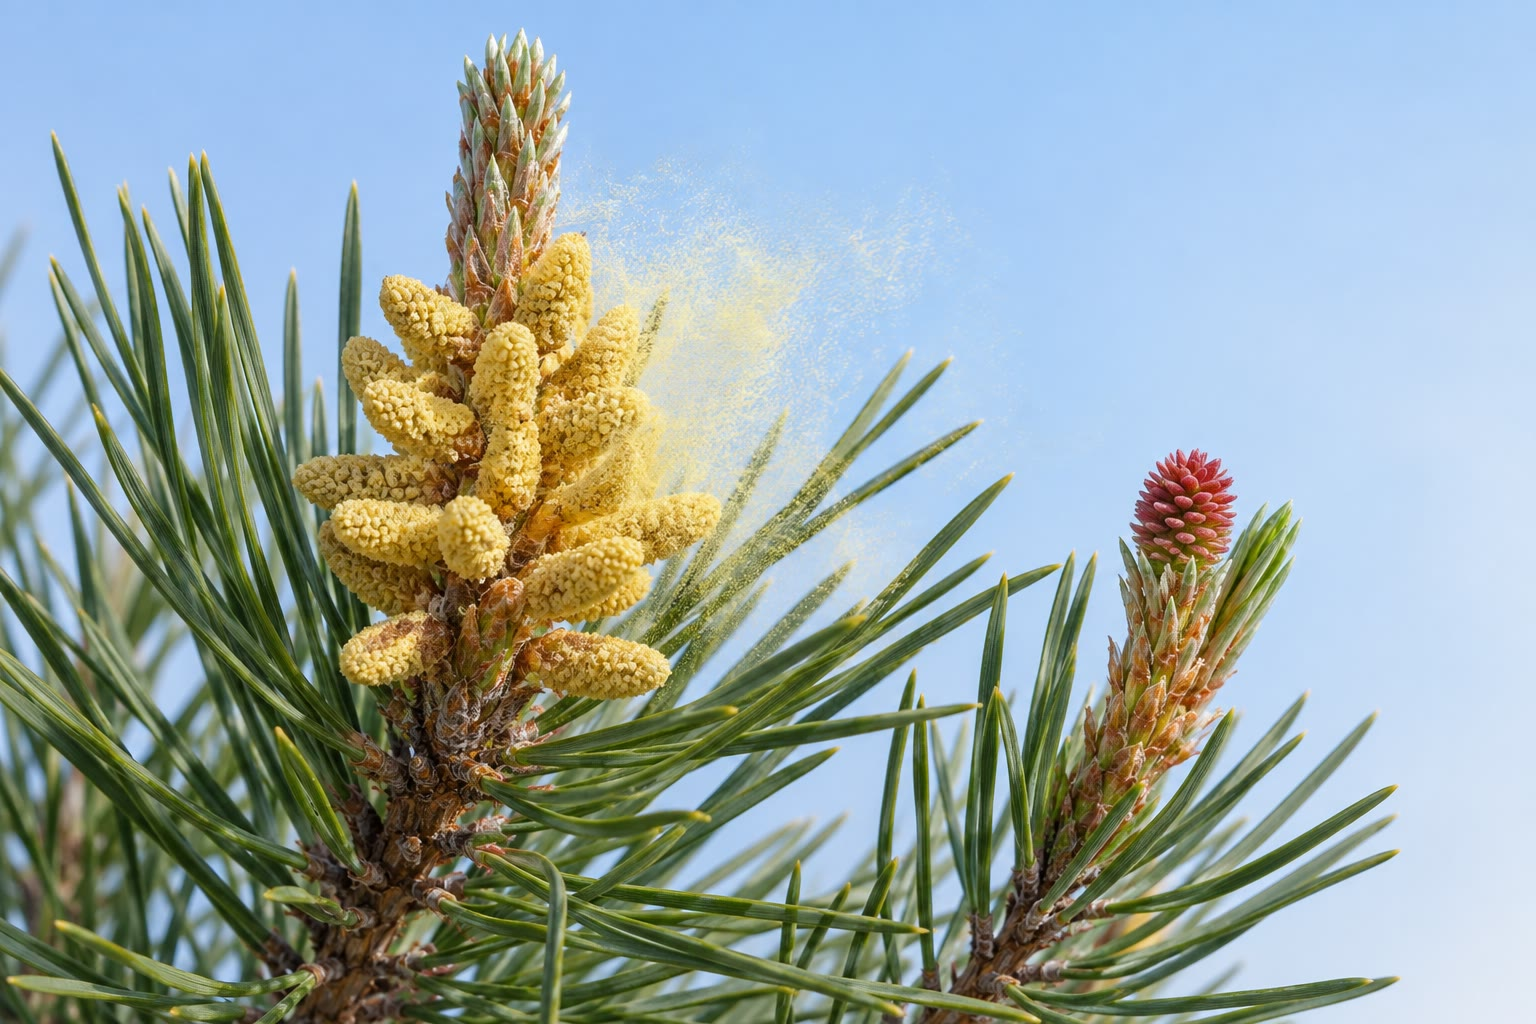
\includegraphics[width=0.6\linewidth]{images/book4/ai/b4-05-pine-cones.jpg}

{\small Un brote de pino en primavera: un grupo de conos masculinos
amarillos que liberan \omterm{def:b2:plant-life-cycles:heterospory}{polen} y, en el extremo de otro brote, un pequeño
cono femenino rojo con las escamas abiertas para capturarlo.}
\end{omfigure}

\begin{example}[Polen en el viento]\label{ex:b2:plant-life-cycles:pollen}
Un grano de \omterm{def:b2:plant-life-cycles:heterospory}{polen} de pino, de \qty{50}{\micro m} de diámetro y con dos
sacos aéreos, cae a unos \qty{3}{cm/s}; un árbol grande libera unos
$10^{11}$ granos en una temporada, suficientes para teñir de amarillo los
estanques. La probabilidad de que un grano caiga en un \omterm{def:b2:plant-life-cycles:heterospory}{óvulo} dado es
ínfima, y la estrategia solo funciona por el número: la polinización por
el viento es barata por grano, cara en granos, y está restringida a
plantas que crecen en rodales de su propia especie --- coníferas,
gramíneas, robles. Las plantas con flores
(\cref{ch:b2:angiosperm-reproduction}) encontraron la manera de hacer
llegar el \omterm{def:b2:plant-life-cycles:heterospory}{polen} mediante animales, grano a grano y a la dirección
correcta.
\end{example}

\section{Tendencias en las plantas terrestres}

\begin{proposition}[Cuatro tendencias]\label{prop:b2:plant-life-cycles:trends}
\index{reducción del gametofito}
De los \omterm{def:b2:plant-life-cycles:moss}{musgos} a los \omterm{def:b2:plant-life-cycles:fern}{helechos} y a las plantas con semilla: (1) el
\omterm{def:b2:plant-life-cycles:cycles}{esporofito} pasa de ser un tallito dependiente a ser toda la planta, y el
\omterm{def:b2:plant-life-cycles:cycles}{gametofito} se reduce de planta a lámina y de lámina a unas pocas
células; (2) la homosporia cede el paso a la \omterm{def:b2:plant-life-cycles:heterospory}{heterosporia}, y el
\omterm{def:b2:plant-life-cycles:cycles}{gametofito} femenino permanece sobre la planta madre; (3) la fecundación
pasa de los anterozoides que nadan en el agua superficial a un tubo
polínico, de modo que la reproducción ya no necesita lluvia; (4) la
unidad de dispersión pasa de la espora --- una sola célula con reservas
para un día --- a la semilla, un embrión con alimento y cubierta, que
puede esperar. La generación \omterm{def:b2:meiosis-heredity:meiosis}{diploide} se ve favorecida en tierra firme
porque un cuerpo \omterm{def:b2:meiosis-heredity:meiosis}{diploide} enmascara las \omterm{def:b2:genome-diversification:mutation}{mutaciones} recesivas, puede
crecer más y vivir más tiempo con un sistema vascular, y porque una
espora formada por \omterm{def:b2:meiosis-heredity:meiosis}{meiosis} sobre un \omterm{def:b2:plant-life-cycles:cycles}{esporofito} alto llega más lejos que
un gameto que nada desde un \omterm{def:b2:plant-life-cycles:cycles}{gametofito} bajo. La tendencia continúa en las
plantas con flores, donde el \omterm{def:b2:plant-life-cycles:cycles}{gametofito} femenino tiene siete células y la
semilla está envuelta en un fruto.
\end{proposition}

\begin{example}[Los grupos comparados]\label{ex:b2:plant-life-cycles:table}
\begin{center}
\small
\begin{tabular}{p{2.3cm}p{3.1cm}p{3.1cm}p{3.3cm}}
\hline
 & \omterm{def:b2:plant-life-cycles:moss}{musgos} & \omterm{def:b2:plant-life-cycles:fern}{helechos} & coníferas \\
\hline
generación \omterm{def:b2:meiosis-heredity:vocabulary}{dominante} & \omterm{def:b2:plant-life-cycles:cycles}{gametofito} & \omterm{def:b2:plant-life-cycles:cycles}{esporofito} & \omterm{def:b2:plant-life-cycles:cycles}{esporofito} \\
\omterm{def:b2:plant-life-cycles:cycles}{gametofito} & tallo folioso, cm & \omterm{def:b2:plant-life-cycles:fern}{prótalo}, mm, libre & grano de \omterm{def:b2:plant-life-cycles:heterospory}{polen} (4 células); contenido del \omterm{def:b2:plant-life-cycles:heterospory}{óvulo} (miles de células) \\
esporas & de un tipo & de un tipo & \omterm{def:b2:plant-life-cycles:heterospory}{microsporas}, \omterm{def:b2:plant-life-cycles:heterospory}{megasporas} \\
fecundación & anterozoides nadadores en el agua & anterozoides nadadores en el agua & tubo polínico \\
unidad de dispersión & espora & espora & semilla \\
tejido vascular & ninguno & xilema, floema & xilema, floema, madera \\
\hline
\end{tabular}
\end{center}
\end{example}

\section{Ejercicios}

\begin{exercise}[$\star$]\label{exo:b2:plant-life-cycles:1}
Defínanse \omterm{def:b2:plant-life-cycles:cycles}{gametofito}, \omterm{def:b2:plant-life-cycles:cycles}{esporofito}, espora y gameto, y dígase mediante qué
tipo de división (mitosis o \omterm{def:b2:meiosis-heredity:meiosis}{meiosis}) se produce cada uno de los cuatro.
\end{exercise}

\begin{exercise}[$\star$]\label{exo:b2:plant-life-cycles:2}
El \omterm{def:b2:plant-life-cycles:fern}{helecho} \emph{Ophioglossum reticulatum} tiene \num{1260} cromosomas en
las células de sus hojas. ¿Cuántos hay en una espora, en una célula del
\omterm{def:b2:plant-life-cycles:fern}{prótalo}, en un anterozoide, en una oosfera, en un cigoto?
\end{exercise}

\begin{exercise}[$\star$]\label{exo:b2:plant-life-cycles:3}
¿Qué generación es el cojín verde de un \omterm{def:b2:plant-life-cycles:moss}{musgo}? ¿Y el pedicelo pardo con
una cápsula? ¿Una fronda de \omterm{def:b2:plant-life-cycles:fern}{helecho}? ¿Un \omterm{def:b2:plant-life-cycles:fern}{prótalo}? ¿Un grano de \omterm{def:b2:plant-life-cycles:heterospory}{polen}? ¿La
reserva de alimento de una semilla de pino? ¿El embrión de una semilla
de pino?
\end{exercise}

\begin{exercise}[$\star$]\label{exo:b2:plant-life-cycles:4}
Nómbrense los tres tipos de \omterm{def:b2:plant-life-cycles:cycles}{ciclo de vida} y dese un organismo de cada
uno. ¿Dónde tiene lugar la \omterm{def:b2:meiosis-heredity:meiosis}{meiosis} en cada caso?
\end{exercise}

\begin{exercise}[$\star\star$]\label{exo:b2:plant-life-cycles:5}
Un anterozoide de \omterm{def:b2:plant-life-cycles:moss}{musgo} nada a \qty{100}{\micro m/s}. ¿Cuánto tarda en
alcanzar un \omterm{def:b2:plant-life-cycles:moss}{arquegonio} situado a \qty{3}{cm}? Una película de rocío se
evapora \qty{20}{min} después del amanecer: ¿cuál es el alcance máximo de
la fecundación? Coméntese el tamaño de las colonias de \omterm{def:b2:plant-life-cycles:moss}{musgo}.
\end{exercise}

\begin{exercise}[$\star\star$]\label{exo:b2:plant-life-cycles:6}
Calcúlese la velocidad de sedimentación en el aire de una espora de
\omterm{def:b2:plant-life-cycles:fern}{helecho} de radio \qty{15}{\micro m} y densidad \qty{1100}{kg/m^3} ($\eta =
\qty{1.8e-5}{Pa.s}$, $\rho_{\text{aire}} = \qty{1.2}{kg/m^3}$), y la
distancia que recorre desde \qty{0.5}{m} con un viento de \qty{2}{m/s}.
Rehágase para una semilla de pino de \qty{5}{mg} de masa cuya ala le da
una velocidad de descenso de \qty{0.8}{m/s}, liberada desde \qty{20}{m}.
\end{exercise}

\begin{exercise}[$\star\star$]\label{exo:b2:plant-life-cycles:7}
Una fronda de \omterm{def:b2:plant-life-cycles:fern}{helecho} lleva \num{200} \omterm{def:b2:plant-life-cycles:fern}{soros} de \num{40} \omterm{def:b2:plant-life-cycles:fern}{esporangios}, y
cada \omterm{def:b2:plant-life-cycles:fern}{esporangio} forma \num{64} esporas. ¿Cuántas esporas hay por fronda?
Si una espora de cada $10^{5}$ da un \omterm{def:b2:plant-life-cycles:fern}{prótalo} y un \omterm{def:b2:plant-life-cycles:fern}{prótalo} de cada
\num{50} produce un \omterm{def:b2:plant-life-cycles:cycles}{esporofito}, ¿cuántos \omterm{def:b2:plant-life-cycles:fern}{helechos} jóvenes rinde una
fronda?
\end{exercise}

\begin{exercise}[$\star\star$]\label{exo:b2:plant-life-cycles:8}
Explíquese por qué la \omterm{def:b2:plant-life-cycles:heterospory}{heterosporia} es una condición previa de la semilla,
y por qué una planta homospórica no podría encerrar su \omterm{def:b2:plant-life-cycles:cycles}{gametofito}
femenino en un \omterm{def:b2:plant-life-cycles:heterospory}{óvulo}.
\end{exercise}

\begin{exercise}[$\star\star$]\label{exo:b2:plant-life-cycles:9}
Compárense una espora de \omterm{def:b2:plant-life-cycles:fern}{helecho} (una esfera de radio \qty{15}{\micro m}
y densidad \qty{1100}{kg/m^3}) y una semilla de pino (\qty{5}{mg}) como
unidades de dispersión: masa, contenido energético (tómense
\qty{20}{kJ/g} de materia seca y un \qty{50}{\%} de materia seca), y lo
que cada una puede y no puede hacer al llegar al suelo.
\end{exercise}

\begin{exercise}[$\star\star\star$]\label{exo:b2:plant-life-cycles:10}
Un pino libera $10^{11}$ granos de \omterm{def:b2:plant-life-cycles:heterospory}{polen} sobre un bosque; a la altura de
los \omterm{def:b2:plant-life-cycles:heterospory}{óvulos}, los granos quedan repartidos en una capa de \qty{20}{m} de
espesor sobre \qty{1}{km^2}. Estímense la concentración de \omterm{def:b2:plant-life-cycles:heterospory}{polen} (granos
por metro cúbico), el número de granos por segundo que atraviesan la
abertura micropilar de un \omterm{def:b2:plant-life-cycles:heterospory}{óvulo} (\qty{0.1}{mm^2}) con un viento de
\qty{2}{m/s}, y el tiempo que tarda un \omterm{def:b2:plant-life-cycles:heterospory}{óvulo} en recibir un grano. ¿Qué
dice esto sobre el momento de apertura de los conos?
\end{exercise}

\begin{exercise}[$\star\star\star$]\label{exo:b2:plant-life-cycles:11}
Dense tres razones por las que la generación \omterm{def:b2:meiosis-heredity:meiosis}{diploide} llegó a dominar el
\omterm{def:b2:plant-life-cycles:cycles}{ciclo de vida} de las plantas terrestres, y una razón por la que la
generación \omterm{def:b2:meiosis-heredity:meiosis}{haploide} no desapareció del todo.
\end{exercise}

\begin{exercise}[$\star\star\star$]\label{exo:b2:plant-life-cycles:12}
Hofmeister trabajó antes de que se conocieran los cromosomas. Explíquese
qué pudo y qué no pudo establecer sobre la \omterm{def:b2:plant-life-cycles:cycles}{alternancia de generaciones}
solo con el microscopio y el cultivo, y qué añadieron los recuentos de
cromosomas.
\end{exercise}

\section{Problema: de la espora a la semilla}

\begin{problem}[{Problema de fin de semana --- se compara la aritmética
reproductiva de un helecho y de un pino, desde el número de esporas y de
granos de polen hasta su dispersión, el destino de los gametofitos y el
coste de una semilla, hasta llegar al número de propágulos que cada
planta debe producir para lograr un solo reemplazo}]
\label{pb:b2:plant-life-cycles:1}
Un \omterm{def:b2:plant-life-cycles:fern}{helecho} lleva \num{10} frondas fértiles, cada una con \num{200}
\omterm{def:b2:plant-life-cycles:fern}{soros} de \num{40} \omterm{def:b2:plant-life-cycles:fern}{esporangios} que forman \num{64} esporas cada uno.
Esporas: radio \qty{15}{\micro m}, densidad \qty{1100}{kg/m^3}. Un pino
produce a lo largo de su vida \omterm{def:b2:plant-life-cycles:heterospory}{óvulos} equivalentes a $2\times 10^{4}$ conos
femeninos ---
tómense \num{100} \omterm{def:b2:plant-life-cycles:heterospory}{óvulos} por cono --- y $10^{11}$ granos de \omterm{def:b2:plant-life-cycles:heterospory}{polen}
al año. Semillas: \qty{5}{mg}, con un \qty{50}{\%} de materia seca a
\qty{20}{kJ/g}. Aire: $\eta = \qty{1.8e-5}{Pa.s}$, $\rho =
\qty{1.2}{kg/m^3}$; $g = \qty{9.81}{m/s^2}$.

\medskip
\noindent\textbf{Parte I --- Las esporas del \omterm{def:b2:plant-life-cycles:fern}{helecho}.}
\begin{enumerate}
  \item Calcúlese el número de esporas que libera la planta en una
        temporada.
  \item Calcúlense la masa de una espora y la de toda la cosecha.
  \item Calcúlese la velocidad de sedimentación de la espora en el aire.
  \item Desde frondas a \qty{0.5}{m}, con un viento de \qty{1.5}{m/s},
        ¿qué distancia recorren las esporas? ¿Sobre qué superficie (un
        disco de ese radio) se reparten, y cuántas caen por metro
        cuadrado?
  \item Explíquese por qué la turbulencia lleva unas pocas esporas mucho
        más lejos, y qué implica esto para la colonización de una isla
        nueva.
  \item Calcúlese el contenido energético de una espora (\qty{50}{\%} de
        materia seca a \qty{20}{kJ/g}) y el de toda la cosecha, y
        compárese con la energía de una semilla de pino.
\end{enumerate}

\medskip
\noindent\textbf{Parte II --- Los \omterm{def:b2:plant-life-cycles:cycles}{gametofitos}.}
Una espora de cada $2\times 10^{4}$ cae en un suelo lo bastante húmedo
para dar un \omterm{def:b2:plant-life-cycles:fern}{prótalo}; un \omterm{def:b2:plant-life-cycles:fern}{prótalo} vive \num{6} semanas y necesita una noche
húmeda --- probabilidad de $0.2$ por semana --- para la fecundación; un
\omterm{def:b2:plant-life-cycles:fern}{prótalo} fecundado da un \omterm{def:b2:plant-life-cycles:cycles}{esporofito} joven con probabilidad
$0.5$; un \omterm{def:b2:plant-life-cycles:cycles}{esporofito} joven sobrevive hasta la edad adulta con probabilidad
$0.02$.
\begin{enumerate}[resume]
  \item ¿Cuántos \omterm{def:b2:plant-life-cycles:fern}{prótalos} produce la cosecha de la planta?
  \item Calcúlese la probabilidad de que un \omterm{def:b2:plant-life-cycles:fern}{prótalo} tenga al menos una
        noche húmeda en sus seis semanas.
  \item Calcúlese el número esperado de \omterm{def:b2:plant-life-cycles:fern}{helechos} adultos que produce la
        cosecha de una temporada.
  \item Si el progenitor vive \num{30} años, ¿cuántos descendientes
        adultos deja, y qué dice esto de la población de \omterm{def:b2:plant-life-cycles:fern}{helechos}?
  \item Un anterozoide de \omterm{def:b2:plant-life-cycles:fern}{helecho} nada a \qty{100}{\micro m/s} y los
        \omterm{def:b2:plant-life-cycles:moss}{arquegonios} de un \omterm{def:b2:plant-life-cycles:fern}{prótalo} están a \qty{1}{mm} de sus propios
        \omterm{def:b2:plant-life-cycles:moss}{anteridios}. ¿Cuánto tarda la autofecundación? ¿Por qué muchos
        \omterm{def:b2:plant-life-cycles:fern}{helechos} la evitan pese a todo (dese un mecanismo)?
  \item ¿En qué sentido es el \omterm{def:b2:plant-life-cycles:fern}{prótalo} el eslabón débil del ciclo del
        \omterm{def:b2:plant-life-cycles:fern}{helecho}?
\end{enumerate}

\medskip
\noindent\textbf{Parte III --- El \omterm{def:b2:plant-life-cycles:heterospory}{polen} del pino.}
\begin{enumerate}[resume]
  \item Un grano de \omterm{def:b2:plant-life-cycles:heterospory}{polen} es una esfera de radio \qty{25}{\micro m} y de
        densidad efectiva \qty{600}{kg/m^3} (sacos aéreos incluidos).
        Calcúlese su velocidad de sedimentación.
  \item Desde un cono a \qty{15}{m}, con un viento de \qty{3}{m/s}, ¿qué
        distancia recorre?
  \item Los $10^{11}$ granos se reparten por \qty{1}{km^2} de bosque
        hasta una altura de \qty{20}{m}. Calcúlese la concentración.
  \item Un micrópilo presenta una abertura de \qty{0.1}{mm^2} a un viento
        de \qty{2}{m/s}. Calcúlense el número de granos que entran en él
        por hora y el tiempo que tarda en recibir el primer grano.
  \item Explíquese por qué un pino aislado a \qty{5}{km} del bosque casi
        no produce semillas, y por qué las especies polinizadas por el
        viento crecen en rodales.
  \item Compárense las cifras: ¿cuántos granos de \omterm{def:b2:plant-life-cycles:heterospory}{polen} produce el bosque
        por \omterm{def:b2:plant-life-cycles:heterospory}{óvulo}, si tiene \num{1000} pinos con \num{2000} \omterm{def:b2:plant-life-cycles:heterospory}{óvulos} cada
        uno?
\end{enumerate}

\medskip
\noindent\textbf{Parte IV --- Las semillas del pino.}
De los \omterm{def:b2:plant-life-cycles:heterospory}{óvulos} del árbol, el \qty{60}{\%} se poliniza y el \qty{80}{\%} de
estos forma una semilla; una semilla da una plántula con probabilidad
$0.05$, y una plántula llega a adulta con probabilidad $0.01$.
\begin{enumerate}[resume]
  \item Calcúlense el número de semillas que produce el árbol a lo largo
        de su vida, y su masa y su energía totales.
  \item Una semilla alada desciende a \qty{0.8}{m/s}. Desde \qty{20}{m},
        con un viento de \qty{3}{m/s}, ¿qué distancia recorre? Compárese
        con el \omterm{def:b2:plant-life-cycles:heterospory}{polen}.
  \item Calcúlese el número esperado de descendientes adultos, y
        compárese con el del \omterm{def:b2:plant-life-cycles:fern}{helecho}.
  \item Calcúlese la energía que invierte el árbol por descendiente
        adulto, y la del \omterm{def:b2:plant-life-cycles:fern}{helecho} por descendiente adulto (solo en
        esporas), y compárense.
  \item La espora de \omterm{def:b2:plant-life-cycles:fern}{helecho} puede esperar unas pocas semanas; la semilla
        de pino, varios años. Explíquese, con las cifras de energía, por
        qué la semilla puede permitirse la latencia y la espora no.
  \item Dense dos ventajas que hacen que la semilla compense su coste y
        dos condiciones en las que la estrategia del \omterm{def:b2:plant-life-cycles:fern}{helecho} es la mejor.
  \item Enúnciese el resultado: propágulos por descendiente adulto para
        el \omterm{def:b2:plant-life-cycles:fern}{helecho} y para el pino, y la energía que cada uno gasta por
        descendiente adulto.
\end{enumerate}
\end{problem}
